% !Mode:: "TeX:UTF-8"
% !TeX program = lualatex

\documentclass[a4paper, 9pt, twocolumn]{extarticle}
\usepackage[dvips]{graphicx}		
\usepackage{tabularx}
\usepackage{multirow}	
\usepackage{url}
%\usepackage[ansinew]{inputenc}
\usepackage{fontspec} %LuaLaTeX
\usepackage{parskip}
\usepackage{amsmath}

% \usepackage[]{auto-pst-pdf}
% \usepackage{pstricks}
% \usepackage{pst-plot}
% \usepackage{pst-node}
% \usepackage{multido}
% \usepackage{url}


\addtolength{\textwidth}{2.1cm}
\addtolength{\topmargin}{-2.4cm}
\addtolength{\oddsidemargin}{-1.1 cm}
\addtolength{\textheight}{4.5cm}
\setlength{\columnsep}{0.7cm}

% User defined macros
\def\x{{\mathbf x}}
\def\L{{\cal L}}
\def\SM{{\mathcal S}}
\def\SMO{{\mathcal S^{\mathrm{chroma}}}}
\def\SMS{{\mathcal S^{\mathrm{enh}}}}
\def\SMP{{\mathcal S^{\mathrm{path}}}}
\def\SMPI{{\mathcal S^{\mathrm{struct}}}}
%\def\SMPC{{\mathcal S^{\mathrm{pc}}}}
\def\SMPC{{\mathcal S^{\mathrm{pb}}}}

\pagestyle{empty}

\begin{document}

\date{\normalsize \today}

\title{\vspace{-8mm}\textbf{\Large
Music Structure Analysis Summary\footnote{This is the summary for the reading assignment,
which is part of the exercise of the lecture \emph{Music Processing Analysis}, Winter Term 2015/16,
Friedrich-Alexander Universit\"at Erlangen-N\"urnberg.
Instructor: Prof.\ Dr.\ Meinard M\"uller,
Tutor: Dipl.-Ing. Stefan Baalke.
}}}

% Hier die Namen und Daten der beteiligten Autoren eintragen
\author{
{
\begin{minipage}[t]{.45\textwidth}
\center
Arnulf Becker\\
\small
Friedrich-Alexander Universit\"at Erlangen-N\"urnberg
\protect\\{} % 
\url{arnulf.becker@FAU.de}
\end{minipage}%
\begin{minipage}[t]{.45\textwidth}
\center
Iñigo Fernandez\\%				Iñigo Fernandez\\
\small
Friedrich-Alexander Universit\"at Erlangen-N\"urnberg
\protect\\{} % 
\url{inigo.fernandez@FAU.de}
\end{minipage}%
}
}
 
\maketitle
\thispagestyle{empty}

%%%%%%%%%%%%%%%%%%%%%%%%%%%%%%%%%%%%%%%%%%%%%%%%%%%%%%%%%%%%%%%%%%%%%%%%%%%%%%
\section{Introduction}
\label{section:introduction}
%%%%%%%%%%%%%%%%%%%%%%%%%%%%%%%%%%%%%%%%%%%%%%%%%%%%%%%%%%%%%%%%%%%%%%%%%%%%%%

This is a \LaTeX-template for the summary of the reading assignment summary. Note that the summary
itself should not exceed one page. Furthermore, please provide your feedback concerning the 
book chapter and the lecture on additional pages.
The style of this template may not be changed.



%%%%%%%%%%%%%%%%%%%%%%%%%%%%%%%%%%%%%%%%%%%%%%%%%%%%%%%%%%%%%%%%%%%%%%%%%%%%%%
\section{Main Section}
\label{section:main}
%%%%%%%%%%%%%%%%%%%%%%%%%%%%%%%%%%%%%%%%%%%%%%%%%%%%%%%%%%%%%%%%%%%%%%%%%%%%%%

The summary should consist of one to three main sections.
Please restrict yourself to describing only the the most
important points covered in the chapter. These sections
should contain the motivation of the problem as well as
the most important technical details. Use an easy to read
language with short, clear sentences. 

%%%%%%%%%%%%%%%%%%%%%%%%%%%%%%%%%%%%%%%%%%%%%%%%%%%%%%%%%%%%%%%%%%%%%%%%%%%%%%
% Here you find some additional LaTex code fragments for including figures and
% references which you may find helpful.
%%%%%%%%%%%%%%%%%%%%%%%%%%%%%%%%%%%%%%%%%%%%%%%%%%%%%%%%%%%%%%%%%%%%%%%%%%%%%%

Example for a citation: \cite{Mueller07_InformationRetrieval_SPRINGER}.

Example for figure: Figure~\ref{figure:example}.

\newpage

%%%%%%%%%%%%%%%%%%%%%%%%%%%%%%%%%%%%%%%%%%%%%%%%%%%%%%%%%%%%%%%%%%%%%%%%%%%%%%
\section{Feedback}
\label{section:feedback}
%%%%%%%%%%%%%%%%%%%%%%%%%%%%%%%%%%%%%%%%%%%%%%%%%%%%%%%%%%%%%%%%%%%%%%%%%%%%%%


%-----------------------
% \begin{figure}[t]
% \begin{center}
% 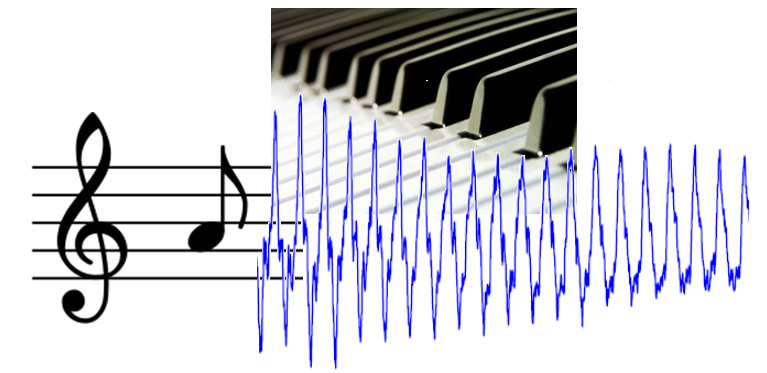
\includegraphics[width=5cm]{figure_example.png}
% \end{center}
% \caption{
% Example for a figure.
% }
% \label{figure:example}
% \end{figure}
%-----------------------


Feedback may also be given in form of bullet points
\begin{itemize}
\item This was good....
\item I did not like...
\end{itemize}



%%%%%%%%%%%%%%%%%%%%%%%%%%%%%%%%%%%%%%%%%%%%%%%%%%%%%%%%%%%%%%%%%%%%%%%%%%%%%%%%%%%%%%%%%%%%%%%%%%
\bibliographystyle{abbrv}
\small
\bibliography{references}
%%%%%%%%%%%%%%%%%%%%%%%%%%%%%%%%%%%%%%%%%%%%%%%%%%%%%%%%%%%%%%%%%%%%%%%%%%%%%%%%%%%%%%%%%%%%%%%%%%



\end{document}

